\begin{comment}
\subsection{Background and Preliminaries}
\label{chap03s1:sec:background}
In this section, we provide the reader with a detailed background on YouTube's video streaming strategy.
{\bf Evolution of YouTube's playback mechanism:} Since its inception in $2005$, viewing videos on YouTube required the Adobe Flash plug-in to be installed on the user's browser\footnote{\url{http://news.bbc.co.uk/2/hi/8287239.stm}}.
In an attempt to reduce third party dependency, and to take advantage of the HTML5 standard which allowed embedded multimedia, YouTube launched an experimental version of the site in January $2010$.
The service, which encompassed only a section of available videos, was extended to users who opted-in for the trial\footnote{\url{https://www.youtube.com/html5}} and were on a browser which supported HTML5 video using WebM or H.264 formats.
YouTube experimented with {\it Dynamic Adaptive Streaming over HTTP (DASH)} around 2013\footnote{\url{https://www.youtube.com/watch?v=UklDSMG9ffU}} to elevate quality of experience of viewers, before adopting it as the default playback mechanism on January 27, 2015\footnote{\url{https://arstechnica.com/gadgets/2015/01/youtube-declares-html5-video-ready-for}\\\url{-primetime-makes-it-default/}}.

\begin{figure}[!t]
 \centering
 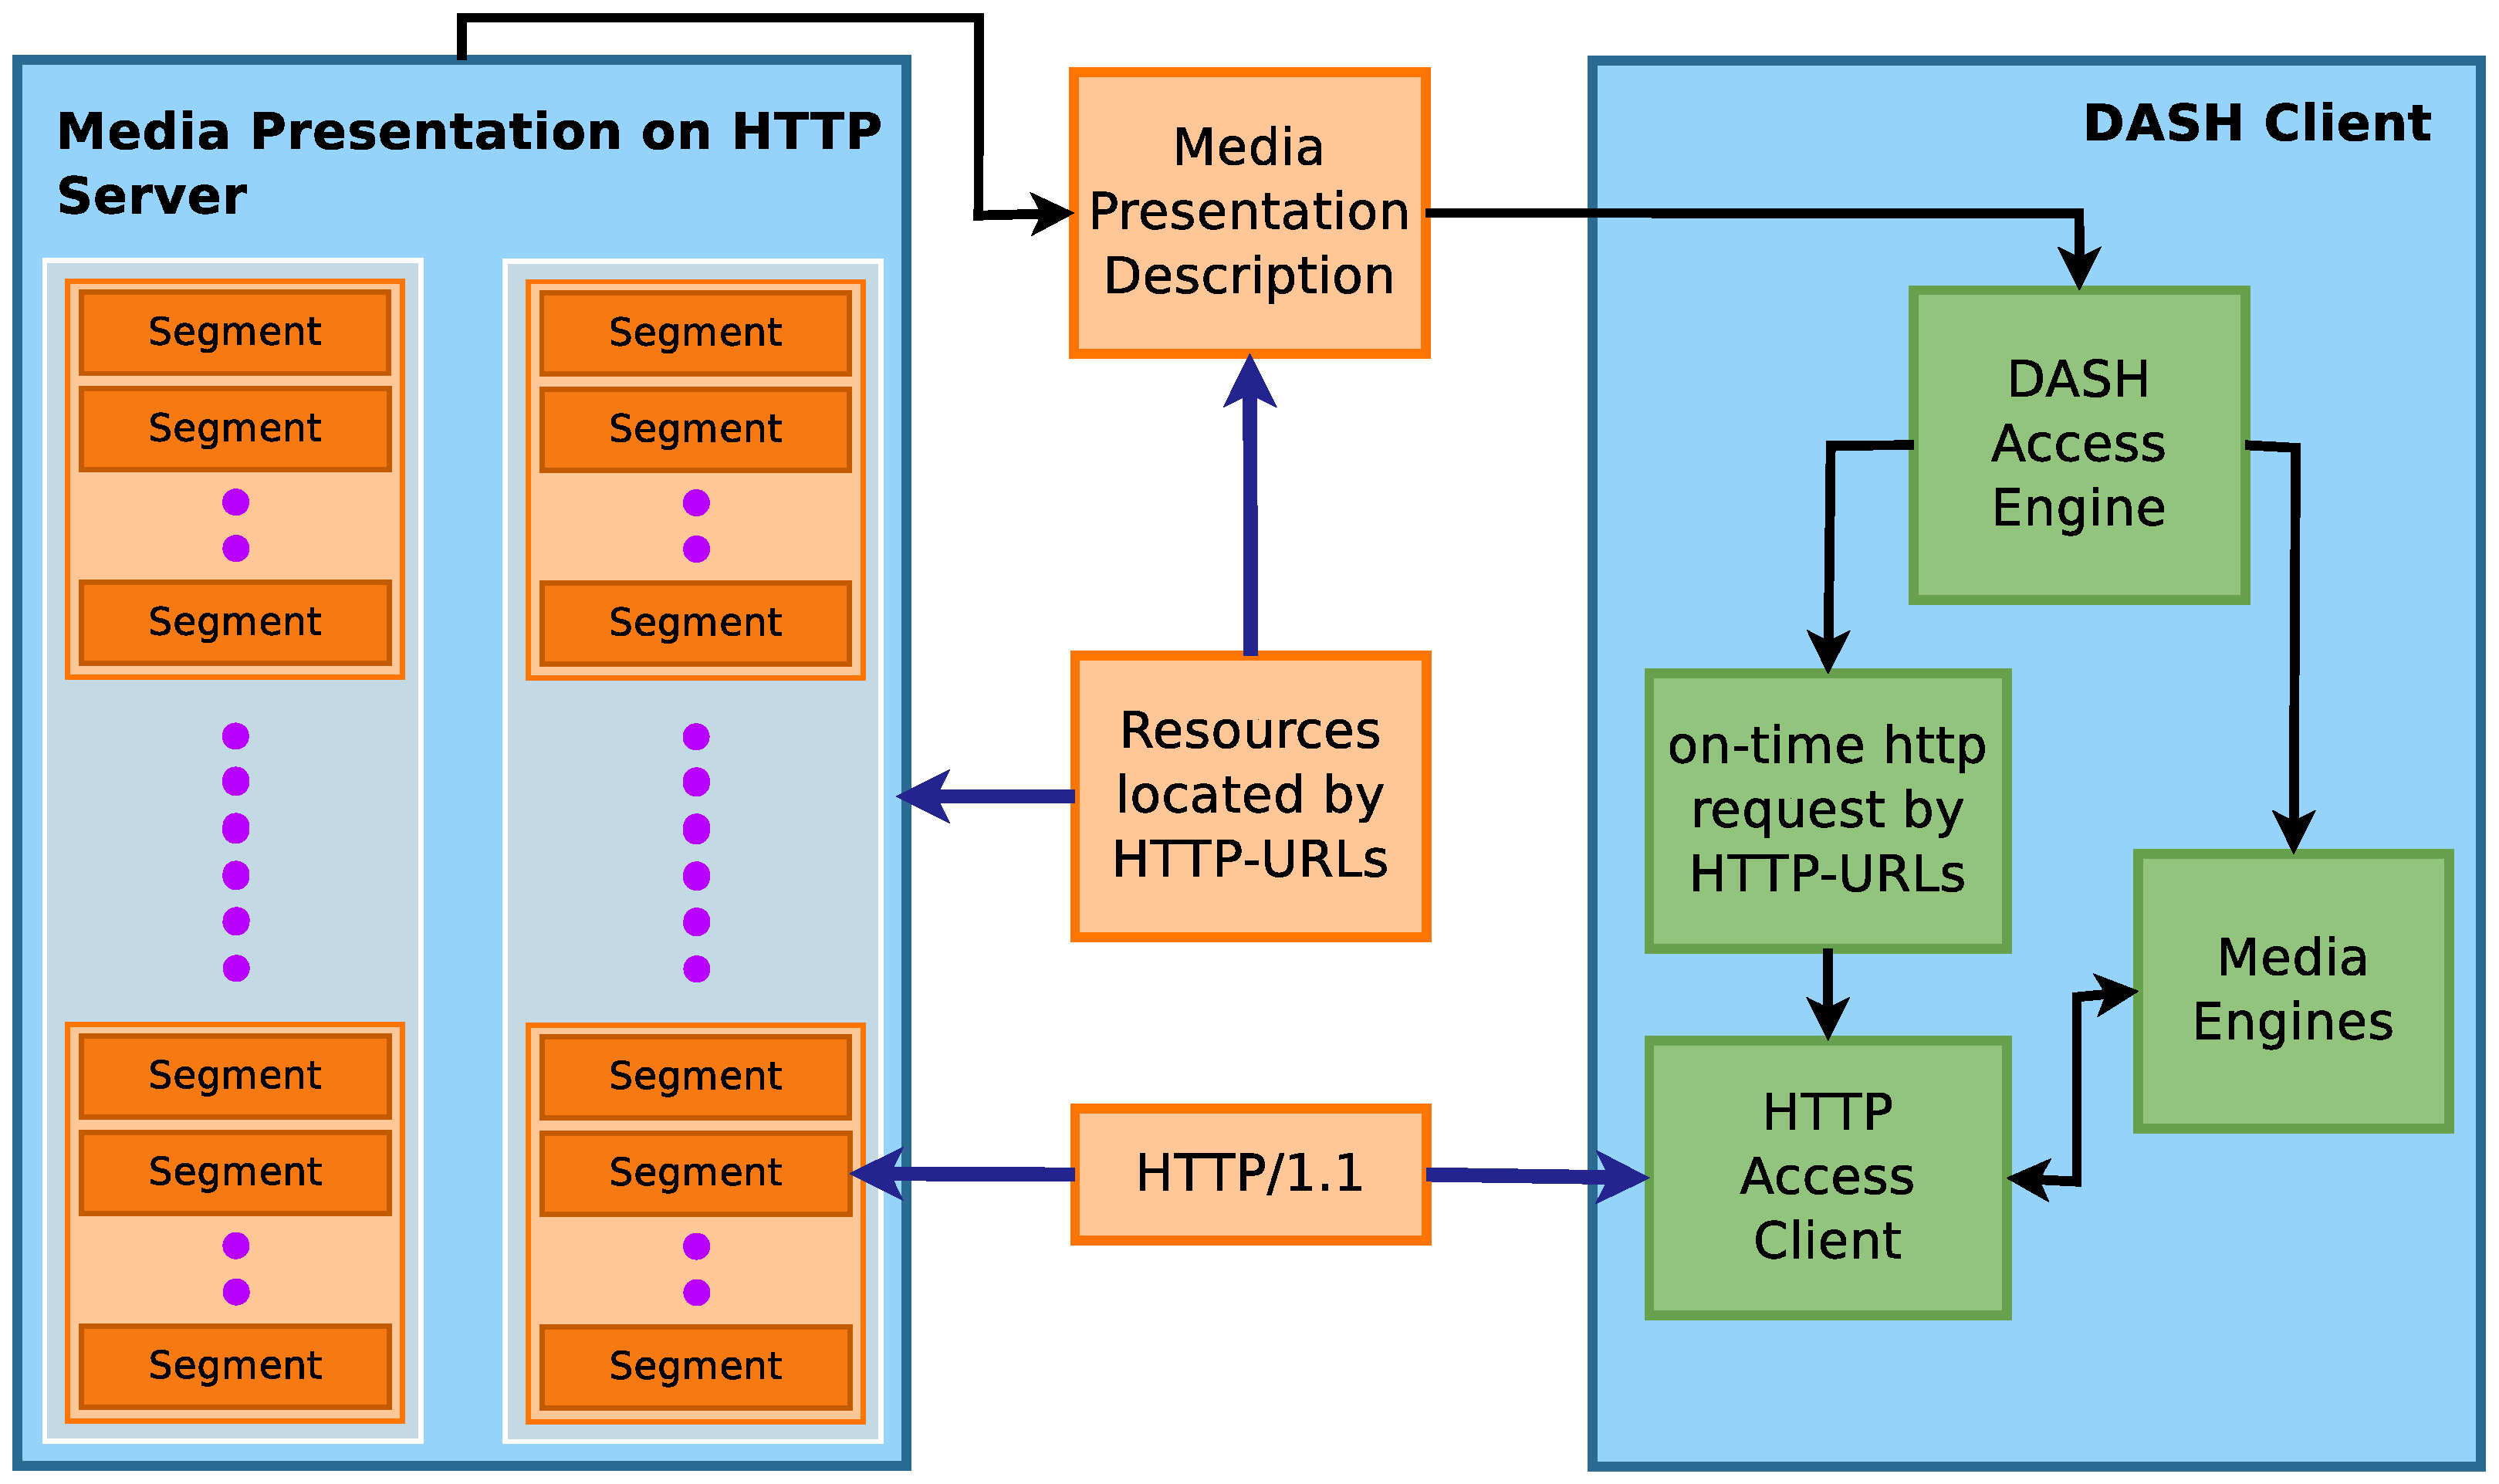
\includegraphics[width=0.7\linewidth]{img/dash-arch}
 \caption{\small{DASH Architecture -- On the left side, the server-side media storage is shown, where content is divided into small segments of alternative bit-rates. On the right side, the DASH client architecture is shown; the {\it DASH Access Engine} monitors network bandwidth at the client and accordingly decides which segment to request from the server. (Image Source: https://www.w3.org/2011/09/webtv/slides/W3C-Workshop.pdf)}}
 \label{fig:chap03s1:dash}
\end{figure}
{\bf DASH specifications:} Dynamic Adaptive Streaming over HTTP (DASH), also referred to as MPEG-DASH, is an adaptive bit-rate solution for video streaming, which enables client-operated video delivery over HTTP.
DASH is implemented by breaking down the video content into small segments, each worth a short duration of playback time.
For every segment of playback time, alternative versions at various bit-rates are available at the server.
The client typically requests for the highest quality segment possible under current network conditions, such that it is received (downloaded) in time for playback, without causing stalling or re-buffering. 
However, DASH is not a protocol -- it only specifies an architecture (Fig.~\ref{fig:chap03s1:dash}) to enable adaptive video streaming over HTTP.
Every video streaming service (e.g., YouTube, Netflix, etc.) is free to define its own implementation of the DASH modules.
In this work, our aim is to study in depth YouTube's implementation of the {\it DASH Access Engine} module (as seen in Fig.~\ref{fig:chap03s1:dash}).

{\bf Encoding technique:} YouTube uses the VP9 codec\footnote{\url{https://youtube-eng.googleblog.com/2015/04/vp9-faster-better-buffer-free-youtube.html}}, which is a free video codec developed by Google to serve YouTube video.
The codec specifies that video files encoded using it shall consist of two types of frames -- (1) key-frame, and (2) intra-frame; key-frames contain complete frame information, while every subsequent intra-frame contains incremental information relative to the last seen key-frame.
Such specifications mandate that a VP9 decoder can start decoding only at key-frames, an observation we utilize to model data consumption more accurately in \S\ref{chap03s1:sec:model}.

{\bf Related Works:} Existing studies on YouTube streaming and quality of experience (QoE) can be grouped into two broad classes.
The first class of works explore traffic patterns and video QoE properties of YouTube~\cite{gill2007youtube,krishnappa2013dashing,wamser2016modeling,wamser2015poster,6757893ieeeexp,7129790ieeeexp}.
These papers mostly study YouTube behavior at the periphery, which although provides a summary of performance metrics, but fails to say much about the internals of YouTube's video streaming protocol.
The second class of studies, however, explore adaptive streaming characteristics of YouTube.
In \cite{finamore2011youtube}, the authors investigate YouTube's data delivery system from the end user view, and illustrate evidence of massive wastage of downloaded data, since viewers often do not watch entire videos -- the study, however, was performed at a time when YouTube used progressive download as the streaming mechanism, and is therefore stale.
\cite{krishnappa2013dashing} is probably the first work to evaluate YouTube's performance since its adoption of adaptive streaming -- the authors claim that YouTube gains $83\%$-$95\%$ in terms of bandwidth by switching from progressive download to DASH.
Some recent works~\cite{sieber2015cost,seufert2015youtube,sieber2016sacrificing} study YouTube's DASH behavior to analyze the trade-off between quality and data wastage -- however, as already pointed out in~\S\ref{chap03s1:sec:introduction}, their approximations lead to gross overestimation. they perform controlled experiments by varying the underlying link bandwidth, and compute wastage.

\end{comment}
